\documentclass[twosided,a4,10pt]{article}
\usepackage[utf8]{inputenc}
\usepackage{amsmath}
\usepackage{amsfonts}
\usepackage{amssymb}
\usepackage{textcomp}
\usepackage{german}
\usepackage{graphicx}
\usepackage[usenames,dvipsnames]{xcolor}
\usepackage{pifont}
\usepackage{nicefrac}
\usepackage{sectsty}
\usepackage{lipsum}  

% ------
% Fonts and typesetting settings
\usepackage[sc]{mathpazo}
\usepackage[T1]{fontenc}
\linespread{1.1} % Palatino needs more space between lines
\usepackage{microtype}
\subsectionfont{\fontsize{10}{15}\selectfont}

% ------
% Page layout
\usepackage[hmarginratio=1:1,top=32mm,columnsep=20pt]{geometry}
\usepackage[font=it]{caption}
\usepackage{paralist}
\usepackage{multicol}

% ------
% Abstract
\usepackage{abstract}
	\renewcommand{\abstractnamefont}{\normalfont\bfseries}
	\renewcommand{\abstracttextfont}{\normalfont\small\itshape}


% ------
% Titling (section/subsection)
\usepackage{titlesec}
\renewcommand\thesection{\Roman{section}}
\titleformat{\section}[block]{\large\scshape\centering}{\thesection.}{1em}{}

% ------
% Clickable URLs (optional)
\usepackage{hyperref}

% ------
% Header/footer
\usepackage{fancyhdr}
	\pagestyle{fancy}
%	\fancyhead{}
	\fancyfoot[C]{Wissenschaftliches Seminar WS 2017/18 $\cdot$
          Software Engineering $\cdot$ Prof. Skornia}
	\fancyhead[C]{OTH Regensburg $\cdot$ Fakultät IM \newline \newline } 
	\fancyfoot[RO,LE]{\thepage}



% ------
% Maketitle metadata
\title{\vspace{-5mm}%
	\fontsize{20pt}{10pt}\selectfont
	\textbf{Adventures in Attacking Wind Farm}
	}	
\vspace{-5mm}\date{}
\author{
	\large
       \begin{minipage}[t]{0.33\linewidth}
         \begin{center}
           	\textsc{Butrint Dehari}\\[2mm]
                 \normalsize	Matr.nr: 3118661\\
                 \normalsize
                 \href{mailto:autor1@stud.oth-regensburg.de}
                 {butrint.dehari@st.oth-regensburg.de}      
         \end{center}
       \end{minipage}        
       \begin{minipage}[t]{0.33\linewidth}
         \begin{center}
           	\textsc{Celestin Mouangue}\\[2mm]
                 \normalsize	Matr.nr: 3080216\\
                 \normalsize
                 \href{mailto:autor2@stud.oth-regensburg.de}
                 {autor2@stud.oth-regensburg.de}      
         \end{center}
       \end{minipage}
       \begin{minipage}[t]{0.33\linewidth}
         \begin{center}
           	\textsc{Zhong XU}\\[2mm]
                 \normalsize	Matr.nr: 123456\\
                 \normalsize
                 \href{mailto:autor3@stud.oth-regensburg.de}
                 {autor3@stud.oth-regensburg.de}      
         \end{center}
       \end{minipage}
     }




%%%%%%%%%%%%%%%%%%%%%%%%
\begin{document}

\tableofcontents

\maketitle
\thispagestyle{fancy}

\begin{abstract}
\noindent Here comes the Abstract...
\end{abstract}
	

\begin{multicols}{2}


\section{Chapter 1 : General Introduction}

\cite{author = {Trevor M. Letcher}, title = {Wind Energy Engineering}, journal = {Derp}, year = {2015}, volume = {1}, pages = {567},}
 \subsection{Why Wind Energy?}
 \subsubsection{Climate Change}
 Today we are threatened by global warming and climate change and therefore the energy industry should try to find energy sources free of carbon dioxide pollution and one of the options is generating electricity from wind energy. Wind and solar energy produce only 4\% of the global supply of electricity while coal, the worst fossil fuel polluter, is still the main energy source for generating electricity. So, producing electricity from wind is where we should be working towards in order to avoid any other environmentally unfriendly material for producing electricity. Hopefully with mass production and bigger and more efficient wind turbines, wind energy and other renewable forms of energy will become cheaper and more convenient to use than fossil fuel and therefore become the main source of producing energy.
 \subsubsection{Advantages of Wind Energy}
 Using wind turbines for electricity generation has many advantages and they have been the main reason for their rapid development.
 \begin{description}
 	\item[$\bullet$]
 	 \textit{Provision for a clean source of energy.} Wind energy delivers electricity without producing carbon dioxide. The relatively small amount of GHG emissions is produced in the manufacture and transport of the turbines and blades.
 	\item[$\bullet$] \textit{Sustainability.} Energy is sent to the grid whenever the sun shines and the wind blows and this makes wind a sustainable source of energy and another reason to invest in wind farms.
 	\item[$\bullet$] \textit{Location.} Wind turbines can be erected almost anywhere and often they are not in competition with urban development or other land usage.
 	\item[$\bullet$]
 	\textit{Stability of cost of electricity.} Once the wind farm is in place the cost of electricity to customers should be stable.
 	\item[$\bullet$]
 	\textit{Cost effectiveness.} Due to mass production and improved design, the cost of producing electricity from wind has significantly decreased.
 	\item[$\bullet$]
 	\textit{Creation of jobs and local resources.} Thousands of workers are employed for the different processes like the manufacture process, transport of turbines or erection of turbines. Wind Energy projects can be of great help in developing local resources, labor, capital, and even materials.
 \end{description}
 
 \subsubsection{Challenges facing the Wind Energy} Making use of the power of the wind comes with some challenges.
 \begin{description}
 	\item[$\bullet$]
 	\textit{Sporadicity of wind.} The most important problem with producing electricity from wind is that wind is unpredictable. It may not be blowing when the electricity from the wind farm is needed.  
 	\item[$\bullet$]
 	\textit{Good sites are often in remote locations.} This means that the electricity produced onshore has to be transported from these remote locations along expensive high-voltage cable to reach the customers.
 	\item[$\bullet$]
 	\textit{Noise pollution.} The noise coming from the rotating wind turbine falls exponentially with distance from the tower, and at 500 m the sound level is less than 35 dB which is not very much when normal conversation is rated at 60 dB.
 	\item[$\bullet$]
 	\textit{Turbine blades can damage wildlife.} The turning blades of wind turbines are the cause of more than 33, 000 bird deaths in the United States.
 	\item[$\bullet$]
 	\textit{Safety.} One of the main reasons that wind turbines are erected away from human habitation is because of safety issues. If a blade would come adrift it would cause serious harm to people or animals nearby.
 	\item[$\bullet$]
 	\textit{New and unfamiliar technology.} Most of the general engineers are unfamiliar with the wind turbines and therefore when installing new wind turbines in some rural areas, it is a good practice to have some trained staff around the area, in case of a malfunction.
 	\item[$\bullet$]
 	\textit{Initial cost.} This is the most serious drawback of setting up a new wind farm and also the main reason why many governments offer subsidies.
 	
 	TODO: ADD REFERENCE : Wind Energy Engineering, by Trevor M. Letcher.
 \end{description}

\subsection{Anatomy of a Wind Turbine}
 \subsubsection{Rotors and Blades}
 Und noch etwas Text... \cite{muster} \newline
 The rotor is the element that captures energy from the wind. The efficiency depends on the number of the blades in the rotor, their shape, their length and the speed at which the rotor turns. The modern blades have a similar shape to an airplane wing and therefore the shape creates lift as the wind passes over it. The blade length depends on the size of the turbine, on the specific blade design and on the site where it is going to generate power from the wind. Typically a 3 MW wind turbine might have a 45m blade at one site where the wind regime is very good and 55m blade to produce the same amount of energy at a different site. The tip speed ratio determines the speed at which a wind turbine rotor turns. It should be an optimum so that each blade should pass through the air and the turbulence it creates should have dissipated before the next blade arrives in the same position.
 TODO: ADD REFERENCE : Wind Power Generation by Paul Breeze.
\subsubsection{The Drive Train, Nacelles and Towers}
\begin{description}
\item[$\bullet$] 
The drive train connects the energy capturing rotor of a wind turbine to the generator which produces the unit's electrical power. The drive train is composed of the gearbox and the generator. The gearbox is responsible for connecting the low-speed shaft attached to the turbine blades to the high-speed shaft attached to the generator. The gearbox converts the slow rotation of the outer blades, typically 30-60 rpm, to the roughly 1000-1800 rpm that the generator needs to start producing energy.
\item[$\bullet$] 
The house of all the main components of the machine except the rotor is called a nacelle. The components include the drive shaft, a gearbox, the generator, a brake to stop the turbine rotating in very low or very high winds and a range of hydraulics and servo systems that control the blade pitch, the rotor speed and the orientation of the complete nacelle structure. Nacelles are usually equipped with a helicopter pad to make it easier for the maintenance crew to land on top of the nacelle. This is very useful on offshore where the maintenance can be difficult sometimes. 
\item[$\bullet$] 
The tower's purpose is to raise the rotor so that it's blades are clear off the ground and of any other obstacle. The higher the turbine rotor is mounted, the stronger the wind, so it is better to raise the nacelle on the highest tower possible. Usually a tower's height is two or three times the blade length. There are different types of towers including: tubular steel towers, lattice towers or concrete towers.

TODO: ADD REFERENCE : Wind Power Generation by Paul Breeze, Understanding Wind Power Technology: Theory, Deployment and Optimisation by Alois Schaffarczyk 
\end{description}

\section{Chapter 2 : Wind Farm Infrastructure }
 \subsection{Wind farm power infrastructure}
 \lipsum[1]
 \subsection{Wind farm communication infrastructure}
 \lipsum[1]
 
 
\section{Chapter 3 : Risk Management and Ransom } 
\subsection{Introduction}
An attacker intending to disrupt wind farm operations or damage equipment would concentrate on six types of targets: (i) control networks; (ii) programmable logic/automation controllers; (iii) network devices; (iv) operator stations; (v) engineering workstations; and (vi) historians. The targets may be accessed using several alternative. The main reason is often the money. Most often we use a ransomware with a cryptocurrency. The most famous cryptocurrency is the Bitcoin . Company can protect their systems. But unfortunately the 0 risk don't exist in the world.

\subsection{Definition of Risk Management}
A security risk assessment is an important element in the overall security risk
management process. Security risk management involves the process of ensuring
that the risk posture of an organization is within acceptable bounds as defined by
senior management. Each security breach has a mitigation. Th main problem issue in security in network is that we don't know how an attacker will to invade our system. That's why a security risk assessment allow company to simulate or imagine several kind of attack and see if their system has a failure.\newline
There are four stages of the security risk management process:
(i) security risk assessment; (ii) test and review; (iii) security risk mitigation; and (iv) operational security.
\begin{itemize}
    \item \textbf{Security Risk Assessment} : This is an objective analysis of the effectiveness of the current security controls that protect an organization’s assets and a
    determination of the probability of losses to those assets. A security risk
    assessment reviews the threat environment of the organization, the value of
    assets, the criticality of systems, the vulnerabilities of the security controls,
    the impact of expected losses, and recommendations for additional controls
    to reduce risk to an acceptable level. Based on this information the senior
    management of the organization can determine if additional security
    controls are required.
    \item \textbf{Test and Review} : Security testing is the examination of the security
    controls against the security requirements. Security controls are determined
    during the security risk assessment and tested during security testing efforts.
    Security testing is performed more frequently than security risk assessments.
    \item \textbf{Risk Mitigation} : Risks to an organization’s assets are reduced through
    the implementation of new security controls or the improvement of existing
    controls. Security risk assessments provide information to allow the
    senior management to make risk-based decisions for the development of
    new controls or expenditure of resources on security improvements on existing controls. Security test and review efforts provide information on
    how to keep existing controls up to date. Risk can be mitigated through
    corrections and additional controls or accepted or transferred.
    \item \textbf{Operational Security} : The implementation and operation of most
    security controls are performed by operational personnel. Daily and weekly
    activities such as applying patches, performing account maintenance, and
    providing security awareness training are essential for maintaining an
    adequate security posture.
\end{itemize}

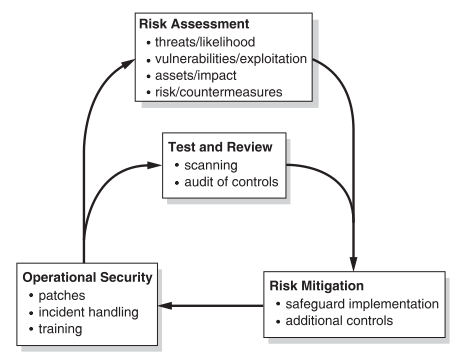
\includegraphics[scale=0.65]{security_management}

\textbf{Add some explication ont these parts.} 
 
 
\subsection{Ransomware and cryptocurrency}
\subsubsection{Ransomware}
Ransomware is a type of malicious software from cryptovirology that threatens to publish the victim's data or perpetually block access to it unless a ransom is paid. While some simple ransomware may lock the system in a way which is not difficult for a knowledgeable person to reverse, more advanced malware uses a technique called cryptoviral extortion, in which it encrypts the victim's files, making them inaccessible, and demands a ransom payment to decrypt them.\newline
There are two main forms of ransomware in circulation today:
\begin{itemize}
    \item Locker ransomware(computer locker):
Denies access to the
computer or device
\item Crypto ransomware
(data locker): Prevents
access to files or data.
\end{itemize}
Crypto ransomware doesn’t necessarily have to use encryption to stop users from accessing their data, but the vast majority of it does. Both types of ransomware are aimed squarely at our digital lifestyle. They are designed to deny us access something we want or need and offer to return what is rightfully ours on payment of a ransom. Despite having similar objectives, the approaches taken by each type of ransomware are quite different.
In our case, the objective is to take control and stop the operation of Windfarm. Then the attacker send a email to demand money via a cryptocurrency like Bitcoin


\subsubsection{cryptocurrency : Bitcoin}

Bitcoin is a collection of concepts and technologies that form the basis of a digital money ecosystem. Units of currency called bitcoins are used to store and transmit value among participants in the bitcoin network. Bitcoin users communicate with each other using the bitcoin protocol primarily via the Internet, although other transport networks can also be used. The bitcoin protocol stack, available as open source software, can be run on a wide range of computing devices, including laptops and smartphones, making the technology easily accessible. \newline
Users can transfer bitcoins over the network to do just about anything that can be done with conventional currencies, including buy and sell goods, send money to people or organizations, or extend credit. Bitcoins can be purchased, sold, and exchanged for other currencies at specialized currency exchanges. Bitcoin in a sense is the perfect form of money for the Internet because it is fast, secure, and borderless.\newline
\newline
Unlike traditional currencies, bitcoins are entirely virtual. There are no physical coins or even digital coins per se. The coins are implied in transactions that transfer value from sender to recipient. Users of bitcoin own keys that allow them to prove ownership of transactions in the bitcoin network, unlocking the value to spend it and transfer it to a new recipient. Those keys are often stored in a digital wallet on each user’s computer. Possession of the key that unlocks a transaction is the only prerequisite to spending bitcoins, putting the control entirely in the hands of each user.\newline
The bitcoin system, unlike traditional banking and payment systems, is based on de-centralized trust. Instead of a central trusted authority, in bitcoin, trust is achieved as an emergent property from the interactions of different participants in the bitcoin system. the transaction is flowing on per-to-per network. It's give a 
complete anonymous. That's why is used
 
\section{Chapter 4 : Security Breach}

\subsection{Introduction}
 According to Staggs, a Ph.D. from University of Tulsa in Tulsa in Oklahoma, There are some vulnerabilities in wind farm nowaday. He listed a overviews of vulnerabilities facing wind farms:
 \begin{itemize}
     \item Programmable automation controllers (PACs) running legacy operating systems, everything is operating as a root, use of insecure remote management services, easy to figure out default passwords, and no code signing
    \item	No authentication or encryption of control messages
    \item	No network segmentation between wind turbines
    \item	No physical security
 \end{itemize}
 Let's talk about some specific attack in the following chapter.


\subsection{Physical Attack}
Five distinct attack vectors are available to target a wind farm control network: cyber access using a wind farm vendor network; cyber access using technician equipment; and cyber via a compromised supply chain, and the most important part in our topic; physical access at a wind turbine, physical access at a substation.
 \subsubsection{Physical access at a wind turbine}
 Wind turbines are generally erected in remote locations with adequate wind speed duration. However, the physical security mechanisms that protect against unauthorized entry inside a wind turbine are fairly simplistic. Typically, the door to a turbine is secured by padlock that can be easily picked or bypassed using bolt cutters. Even if a turbine door has an expensive security mechanism that alert a control center about unauthorized entry, because of the remote location, it may take considerable time for responder to reach the turbine to investigate the unauthorized entry.
 \newline
Once inside the turbine, an attacker could access the wind farm control network by plugging a malicious device such as a Raspberry Pi or a Gustix into network switch. One option is to keep the network configuration intact and insert the malicious device as an additional node in the network. the attacker can use the malicious node to target other nodes in the network. These nodes include other connected turbines and substations. A malicious device configured as a new node in the wind farm control network is susceptible to discovery upon visual inspection as well as over the network. therefore, a more sophisticated access strategy is to position the malicious deice in a man-in-the middle configuration. This involves unplugging a network connection to a trusted device, inserting the malicious device before the device and quickly restoring network connectivity. Implanting the malicious device would cause a temporary disruption, which might be noticed at the transient nature of disruption and timely resumption of network connectivity, it is unlikely that security personnel would immediately trail to the site to investigate the anomaly. A more sophisticated approach is to hide a man-in-the-middle rouge device inside a trusted industrial control system component. This parasitic device drawn power from the same source as the control system component and would be difficult to discover without a detailed inspection involving the removal and disassembly of the control system component. Having gained access to wind farm control network, the attacker could target a variety of information technology and control system assets directly or the attacker could implant malware. The threats include obtaining information about devices, protocols, network configurations and operations; disrupting wind farm operations; and even damaging key physical component, including the wind turbine itself.
 \subsubsection{Physical access at a substation}
 Unlike wind turbines, substations have strong physical security mechanisms such as locks, cameras, motion sensors, remote alerting systems, reinforced constructions and fences. However, substations are still vulnerable to physical penetration and can also be accessed by malicious insiders. Since many substations are located in remote areas and are usually unnamed, it may take some time for security personnel to respond to the site of a breach. Having breached a substation, an attacker can apply the same techniques and tools used to gain access to the wind farm control networks; install persistent, hard-to-discover, parasitic devices; implant malware to surveil and disrupt wind farm operations; and possibly damage or destroy wind farm assets. In fact, unauthorized access to a substation could have more serious implications than a wind turbine breach. This is because the attacker can potentially manipulate the operations controls system as well as the transmission control system.
 \subsubsection{Cyber asses using technician equipment}
 Compromising operator and or service personnel equipment either directly via a flash drive or hands-on access, or indirectly via spear phishing can bridge air-gapped networks. The initial additional tools or malware (for privilege escalation, enhanced access and persistence) to eventually launch attacks against wind turbines and substations. Technicians equipment that could be compromised includes standard laptops, workstations and mobile communications devices. Of a particular interest to attackers are handled devices used by wind farm personnel to performs maintenance on turbine controls systems. This device communicates with a wind turbine control system over a common network medium (RS-232 or ethernet). Compromising such device enables an attacker to target trusted control network assets as well as physical equipment.
 \subsubsection{Cyber access via a compromised supply chain}
 This attack vector can be used to achieved similar access and effects as cyber access using technician equipment. However, in this case, information technology and industrial controls system hardware, firmware and software are compromised in the supply chain, before they are installed at a wind farm
 \newline We can’t talk about the windfarm physical attack without speaking about how to avoid the in another’s words physical security.
 
 \subsubsection{Cyber access using a wind farm vendor network}
 In many cases, wind farm vendors have unfettered remote virtual private network (VPN) access to wind farm control networks for monitoring, software upgrades and maintenance. This access may also be provided to vendors for research and development efforts, especially for evaluating product enhancements. Granting remote access to a wind farm vendor introduces risk and creates disturbing cyber attack environment. This is because the vendor network becomes a single point of access to multiple wind farm deployments, including wind farms belonging to other companies that rely on the vendors for products and services. An attacker could gain access to a vendor network in any number of ways, including via spear phishing campaigns, malicious insiders or physical breaches. After the vendors network is compromised, the attacker can leverage trust relationships to orchestrate attacks on multiple wind farms and their assets. During a security assessment of a wind farm conducted by authors of this paper, a vendor was observed to have remote access (from abroad) to the wind farm operations network. Standard network management protocols were utilized by the vendor, presumably for pushing software upgrades and performing diagnostics. Although the remote vendor communications were encrypted and tunneled over a VPN, the encapsulating protocols were outdated and unencrypted. This could enable a malicious entity to intercept, manipulate and fabricate messages, and launch a slew of attacks against wind turbines, substations and even win farm vendor networks.
 

\subsection{Physical security} 
Perhaps the most significant threat to wind farm is physical access to wind turbines and substations that enables an attacker to target the operations and transmission control networks. As mentioned above, existing physical security mechanisms are relatively weak, and the turbines and substations are typically sanctioned at remote locations. Efforts should be made to outfit every turbine with strong locking mechanisms with multifactor authentication, motion sensors, security cameras and remote alarm notifications system. Additionally, management should assign security personnel who are always ready to respond in a timely manner. Substations are very important components of a wind farm physical breaches of substations can be leveraged to wreak havoc on electricity generation and transmission assets. In addition to locking mechanisms, motion sensors, security cameras and remote alarms, substations should be fortified to the extent possible to defeat breaches of doors, windows, walls and roofs
 
\subsection{Network breach}
 \lipsum[1]



%\section{Chapter 4 : Attack Mitigation }

%\subsection{Introduction}
% \textbf{Talk about the risk which we can prevent}
% \lipsum[1]



%\subsection{Physical Access}
%derpde
% \subsubsection{Access Control}
% \lipsum[1]

 %\subsubsection{Locking System}
 %Und noch etwas Text... \cite{muster} \newline
 %\lipsum[1]
 %\subsubsection{Quick Response}
 %\lipsum[1]

 
%\subsection{Network Mitigation}
% \subsubsection{SSL/TLS}
% \lipsum[1]
% \subsubsection{VPN}
% \lipsum[1]
% \subsubsection{Access restriction}
% \textbf{White List}
% \lipsum[1]
 
%\subsection{Best Practice}
% \lipsum[2]

 
 
\bibliographystyle{lit}
\bibliography{lit}
\end{multicols}

\end{document}



